\section{Juegos olímpicos de invierno}

Algunos datos de las medallas obtenidas por algunos países se encuentran en el siguiente archivo, cortesía de \textit{Winter Olympics Medals}. El archivo .csv (comma separated values) lo puede encontrar en \url{http://winterolympicsmedals.com/medals.csv}. Note que en este caso estará separado por comas (,) y no por (;) como se verá en este ejercicio. Considere el parámetro del método \texttt{.split()} según el archivo que utilice.

Note que los archivos .csv pueden ser abiertos por Excel (en este caso, las columnas de datos se separan por comas o puntos y comas, mientras que las filas se separan por saltos de líneas). Un ejemplo de como se ve el archivo abierto con un bloc de notas y el software Excel se ve a continuación en la figura \ref{fig:csv}.

\begin{figure}[H]
    \centering
    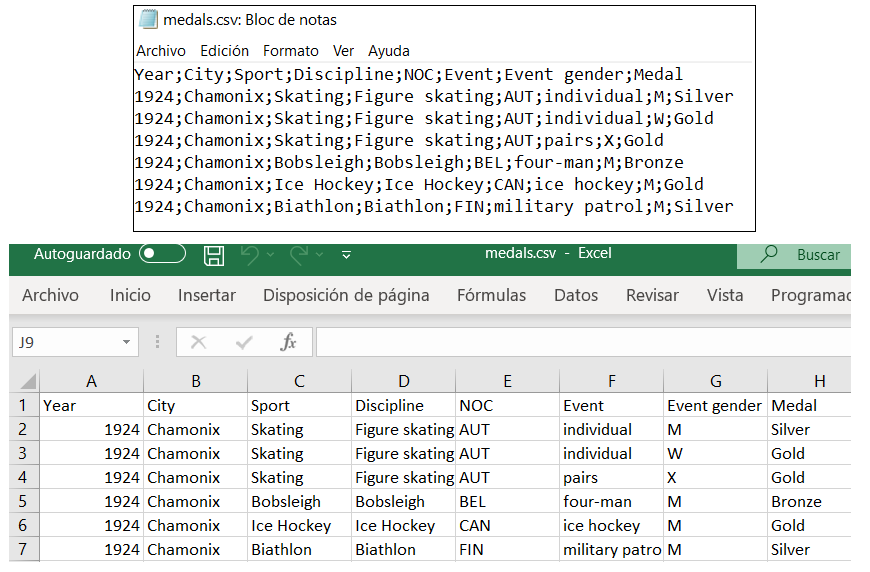
\includegraphics[width=0.7\textwidth]{Guia/csv.png}
    \caption{Diferencias al abrir un archivo csv}
    \label{fig:csv}
\end{figure}

Como comentario, en Chile predeterminadamente se utiliza el punto (.) como separador de miles, la coma (,) como separador decimal y el punto y coma (;) como separador de listas. Si usted utiliza Windows, puede cambiar estas opciones en Panel de control> Reloj y región > Cambiar formatos de fecha, hora o número > Configuración adicional.

En este caso, trabajaremos con Python, por lo que no deberían molestarnos estas diferencias.

El formato del archivo de ejemplo es una fila con los nombres de las columnas \textit{Year, City, Sport, Discipline, NOC, Event gender, Medal}, que se refieren al año de la olimpiada, la ciudad anfitriona, Deporte, Disciplina, Nombre del País, Género de la competencia (M: Masculino, W: Femenino, X: Mixto) y el tipo de Medalla (Gold, Silver y Bronze, referentes a oro plata y bronce).

Su tarea, será completar las funciones que se encuentran en la hoja de trabajo para lograr cumplir con las siguientes tareas.

\begin{itemize}
    \item[a.] \texttt{medallasPorPais(arch\_medallas)} que reciba como parámetro el archivo de texto en formato .csv con la información de las medallas de los juegos. Esta función debe retornar un diccionario donde las llaves sean cada país que se encuentra en el archivo, y los valores una lista de tres enteros con la cantidad de medallas de oro, plata y bronce que ha ganado ese país, respectivamente.
\begin{lstlisting}[style=consola]
>>> [*medallasPorPais('medals.csv')*]
{'AUT': [51, 64, 70], 'BEL': [1, 1, 3], 'CAN': [38, 38, 43] #...}
\end{lstlisting}

    \item[b.] \texttt{paisConMasMedallas(arch\_medallas)} que recibe como parámetro el archivo csv con medallas. Esta función retorne un string con el NOC o abreviatura del país con más medallas ganadas históricamente en los juegos olímpicos de invierno.
\begin{lstlisting}[style=consola]
>>> [*paisConMasMedallas('medals.csv')*]
'NOR'
\end{lstlisting}
    \item[c.] \texttt{cantidadDeJuegos(arch\_medallas)} que al igual que las funciones anteriores, recibe el archivo \texttt{medals.csv} y retorna un entero con la cantidad de juegos olímpicos que se han hecho en el período contemplado por los datos.
\begin{lstlisting}[style=consola]
>>> [*cantidadDeJuegos('medals.csv')*]
20
\end{lstlisting}
    \item[d.] \texttt{escribirResumen(arch\_medallas)} que recibiendo como parámetro los datos del archivo \texttt{medals.csv}, escriba un archivo de texto llamado \texttt{Resumen\_de\_medallas.txt} con la siguiente información. Para ello, complete las variables de la función pre-escrita. Note que esta función retorna nada.
\begin{figure}[H]
    \centering
    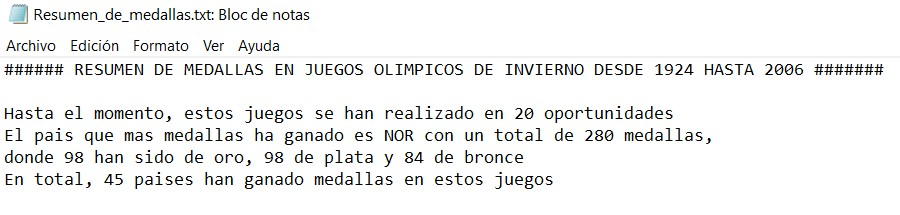
\includegraphics[width=\textwidth]{Guia/resumen.jpg}
\end{figure}
\end{itemize}